\documentclass[../Report.tex]{subfiles}


\begin{document}

\chapter{Iterative Optimierung des Hammerstein-Modells}
\label{chap:opt}

%TODO: überprüfe Referenz zu Jens, da Ideen nicht publiziert wurden! Wie wird das eingebunden?
Ziel der Optimierung von Übertragungsfunktion $\Hcompl$ und Kennlinie $K$ mit ihren Parametern $a$ ist die Minimierung des Fehlers zwischen idealem und gemessenem Ausgangssignal, $\Uout_{, \mathrm{ideal}} \oft$ und $\Uout_{, \mathrm{meas}} \oft$. Die Minimierung des relativen Fehlers ist gegeben durch
\begin{align}
\label{eq:opt.relFehler}
	\min \; \mathit{f} \oft := \min \left( \frac{\Uout_{, \mathrm{meas}} \oft  - \Uout_{, \mathrm{ideal}} \oft}{ \Uout_{, \mathrm{ideal}} \oft} \right) 
	= \min \left( \frac{ \Uout_{, \mathrm{meas}}\oft}{ \Uout_{, \mathrm{ideal}}\oft} -1 \right) 
	\; .
\end{align}
Für das verwendete Hammerstein-Modell liegt die in \cite{harzheim18}
vorgeschlagene getrennte, iterative Optimierung von $\Hcompl$ und $K$ nahe. 
Die Auswertung der Qualität des Einzelsinus erfolgt dabei durch das RF-Tool \cite{RF-Tool} unter Verwendung des als \lstinline{QGesamt1} geführten Qualitätswerts\footnote{\label{foot:opt.H.quality} Hierauf beziehen sich alle weiteren Angaben zur Qualität des Signals. Eine intensivere Befassung mit dem Tool hat nicht stattgefunden.}.
%TODO: Auffüllen Daten!
Dabei wird im Folgenden unter $\Uout_{, \mathrm{ideal}} \oft$ ein durch die Routine \lstinline{generate_BBsignal} erzeugter Einzelsinus betrachtet, vergleiche hierzu \ref{sec:ausb.code}. 

\section{Optimierung der linearen Übertragungsfunktion $H$}
\label{sec:opt.H}

Die Optimierung von $\Hcompl \ofomega$ beruht auf der Annahme, dass sich \eqref{eq:opt.relFehler} auf die komplexen Darstellungen des berechneten und des gemessenen Ausgangssignals $\Uoutc_{, \mathrm{ideal}} \ofomega $ und $\Uoutc_{, \mathrm{meas}} \ofomega $ fortsetzen lässt mit 

\begin{align}
\label{eq:opt.ratio}
	\fabs \ofomega :=  
				\frac{ \Uoutc_{, \mathrm{meas}} \ofomega }{\Uoutc_{, \mathrm{ideal}} \ofomega } -1
				\; .
\end{align}
Ist im Spektrum des gemessenen Signals eine Frequenz verglichen mit dem idealen Signal stärker vertreten, wurde die Verstärkung des realen Systems bei der Berechnung von $\Uquestc$ unterschätzt. Folglich muss die Verstärkung im Hammerstein-Modell angehoben werden. Die Korrektur der Phase ist dabei in \eqref{eq:opt.ratio} mit inbegriffen.
Iterativ mit einer Schrittweite $\sigma_H^i \in \left[ 0 , 1 \right]$ ausgeführt, folgt für den $i$-ten Schritt

\begin{align}
\label{eq:opt.Hnew}
	\Hcompl^{i+1}
		=\Hcompl^{i} \cdot
		\left( 1 + \sigma_H^i \: \fabs^{i}	\right)					 
\end{align}
für $\Uoutc_{, \mathrm{meas}}^{i}$ in $\fabs^{i}$ als gemessenem Ausgangssignal für das mit $\Hcompl^{i}$ berechnete Eingangssignal
\footnote{Nachfolgend wird aus Gründen der Übersichtlichkeit $\fabs$ statt dem länglichen Bruch genutzt.}.
In \figref{fig:opt.spektrum_BB_signal} sind Betrag und Phase der durch FFT erhaltenen Spektren für gemessenes und ideales Ausgangssignal vor Durchführung einer Optimierung dargestellt. Die Transformation erfolgt dabei durch die Erweiterung \lstinline{numpy} in Python mit \lstinline{numpy.fft}. Die Routine nutzt einen Algorithmus von Cooley and Tukey \cite[S. 297-301]{cooley65}.
Klar erkennbar sind die Nulldurchgänge des Betragsspektrums sowie die große Streuung der Phasenwerte. 
%%% TODO: Samples der Signale!
% Insbesondere illustriert \figref{subfig:opt.angle_spektrum} die bei gemessenem Signal auftretende Streuung der Phase. 
\\

\pgfplotstableread[col sep = comma] {opt_spect_ideal_abs.csv} \absSpectIdeal 
\pgfplotstableread[col sep = comma] {opt_spect_meas_abs.csv} \absSpectMeas
\pgfplotstableread[col sep = comma] {opt_spect_ideal_angle.csv} \angleSpectIdeal 
\pgfplotstableread[col sep = comma] {opt_spect_meas_angle.csv} \angleSpectMeas 

\begin{figure}[htb] %%% TODO: prüfen!
\begin{subfigure}{0.5 \textwidth}
\centering
    \begin{tikzpicture}
\begin{axis}[
		legend entries = {Ideales Signal, Gemessenes Signal},
		legend pos = north east,
		xlabel={Frequenz},
		ylabel={Spektraldichte },
		%xtick distance = 10000000,
%		xminorgrids,
%		xmajorgrids,
		minor x tick num =3,
		xtick pos = lower,
		ytick pos = left,
		xtick align = outside,
		ytick align = outside,
		scaled x ticks = base 10:-6,
		xtick scale label code/.code={\si{\MHz}},
		xmin = -5000000,
		xmax = 85000000,
		ymin = 0,
		ymax = 0.03,
		]
		
		\addplot[blue, mark size=3.5pt] table [ x index =0, y index=1] {\absSpectIdeal};	% plot des Idealen Betragsspektrums
		\addplot[orange, mark size=3.5pt] table [ x index =0, y index=1] {\absSpectMeas};	% Plot des gemessenen Betragsspektrums
\end{axis}
\end{tikzpicture}
\caption{Betragsspektren}
	\label{subfig:opt.abs_spektrum}
\end{subfigure}
\begin{subfigure}{0.5 \textwidth}
\centering
    \begin{tikzpicture}
\begin{axis}[
		legend entries = {Ideales Signal, Gemessenes Signal},
		legend pos = north east,
		xlabel={Frequenz},
		ylabel={Phase},
		y label style={at={(axis description cs:-0.1,.5)},anchor=south},
%		%xtick distance = 10000000,
%		xminorgrids,
%		xmajorgrids,
		minor x tick num =3,
		xtick pos = lower,
		ytick pos = left,
		xtick align = outside,
		ytick align = outside,
		scaled x ticks = base 10:-6,
		xtick scale label code/.code={\si{\MHz}},
		xmin = -5000000,
		xmax = 85000000,
		scaled y ticks={real:3.1415},
		ytick scale label code/.code={$\si{\radian}$},
%		ymin = 0,
%		ymax = 0.03,
		]
		
		\addplot[blue, only marks, mark size=1pt] table [ x index =0, y index=1] {\angleSpectIdeal};	% plot des Idealen Betragsspektrums
		\addplot[orange, only marks, mark size=1pt] table [ x index =0, y index=1] {\angleSpectMeas};	% Plot des gemessenen Betragsspektrums
\end{axis}
\end{tikzpicture}
\caption{Phasenspektren}
	\label{subfig:opt.angle_spektrum}
\end{subfigure}
\caption{Spektrum des Einzelsinus-Signals, Berechnung der FFT mit jeweils $109$ Punkten}
\label{fig:opt.spektrum_BB_signal}
\end{figure}

\noindent
Mit diesen Überlegungen gestaltet sich der Programmablauf zur Optimierung der Übertragungsfunktion wie in \figref{fig:Algorithmus.H} illustriert.


\begin{figure}[htb]
\centering
\tikzstyle{block_g} = [rectangle, draw, fill=green!20, 
    text width=6.5em, text centered, rounded corners, node distance=2cm, minimum height=4em]
\tikzstyle{block_b} = [rectangle, draw, fill=blue!20, 
    text width=6em, text centered, rounded corners, node distance=4.5cm, minimum height=4em]
\tikzstyle{block_r} = [rectangle, draw, fill=red!20, 
    text width=6em, text centered, rounded corners, node distance=4.5cm, minimum height=4em]
\tikzstyle{line} = [draw, -latex']
\begin{tikzpicture}[node distance = 5cm, auto]
    % Place nodes
    \node [block_g] (ideal) {$\Uout_{,\textrm{ideal}}$ festlegen};
    \node [block_g, below of=ideal] (H) {$\Hcompl$ bestimmen};
    \node [block_g, below of=H] (K) {$K_0$ bestimmen \newline Ref.: \newline ${V_{PP,?} = \SI{600}{\mV}}$};
    \node [block_b, right of=H] (Uquest) {$\Uquest_{,\textrm{ideal}}$ berechnen};
    \node [block_b, below of=Uquest] (Uin) {$\Uin$ berechnen};
    \node [block_r, right of=Uquest] (adjust) {$\Hcompl$ anpassen $H_i$ neu berechnen};
    \node [block_b, right of=Uin] (Uout) {$\Uout$ messen};
    
    % Draw edges
    \path [line, thick] (ideal) --  (H);
    \path [line, dashed] (H) -- node {$\Hcompl_0$} (Uquest);
    \path [line, thick] (H) -- (K);
    \path [line, thick] (K) -- node {$K$} (Uin);
    \path [line, thick] (Uin) -- (Uout);
	\path [line, thick] (Uout) -- node {$\Uout_{,\textrm{meas}}$}(adjust);
    \path [line, thick] (adjust) -- node {$\Hcompl_i$}(Uquest);
    \path [line, thick] (Uquest) -- (Uin);
    \path [line, dashed] (Uquest) -- ++(0,15mm) -- node {$\Uquest_{,\textrm{ideal}}$} ++(45mm,0) -- (adjust);
\end{tikzpicture}
\caption{Algorithmus zur Optimierung von $\Hcompl$}
  	\label{fig:Algorithmus.H}
\end{figure}



\subsection{Fehlerquellen}
\label{subsec:opt.H.fehler}

Neben den für kontinuierliche Funktionen problemlos definierbaren iterativen Zuweisungen ergeben sich in Messung und diskreter Ausführung jedoch Fehlerquellen. Problematisch sind insbesondere solche, die in \eqref{eq:opt.Hnew} durch das Betragsverhältnis der Ausgangssignale verstärkt werden. 
Unterscheiden sich die Spektren hier um einen großen Faktor, resultiert dies in einer entsprechenden Anpassung der Übertragungsfunktion für die betreffende Frequenz. Dies ist folglich insbesondere bei kleinen Beträgen der Spektren problematisch, wenn Ungenauigkeiten und Störeinflüsse betrachtet werden. 
\\
Besondere Störeinflüsse ergeben sich also durch
\begin{itemize}
	\item Rauschen: Unterschiedliche Rauscharten machen sich in allen Frequenzen bemerkbar mit kritischem Einfluss bei geringer Spektraldichte des Signals.\cite[S. 205 ff.]{lerch10}
	
	\item Diskretisierungsfehler: Die FFT bedingt eine begrenzte Auflösung in den Spektren von $\Hcompl$ und den gemessenen Signalen und liegt im Allgemeinen an unterschiedlichen Frequenzen und mit unterschiedlich vielen Punkten vor.
	
	\item Interpolationsfehler: Die (hier lineare) Interpolation der Spektren zur Auswertung von $\fabs$ an den Frequenzen von $\Hcompl$ kann insbesondere den Einfluss oben genannter Punkte verstärken.
\end{itemize}

\noindent
Weiterhin unterscheidet sich die Auflösung des Spektrums zwischen der FFT der Signale und der Darstellung von $\Hcompl$. Der Frequenzabstand zweier Einträge in den Spektren der Signale ist durch die Wiederholfrequenz $f_{rep}$ gegeben. Hierdurch ergeben sich im betrachteten Bereich der Übertragungsfunktion etwa 100 Werte in den Spektren der Signale, während die Übertragungsfunktion mit über 200 Werten berechnet wird. Hieraus resultiert eine konzeptionelle Ungenauigkeit, auf die in \ref{subsubsec:opt.H.zeropadd} eingegangen wird. 
\\
\\
Ein Aspekt, der sich hierzu in der Implementierung als entscheidend, aber nicht auf den ersten Blick intuitiv darstellt, liegt in der Periodendauer diskreter Signale. Bei diskreten Zeitsignalen ist zu beachten, dass die Periodendauer $T$ nicht durch die Differenz der Zeitwerte des letzten und des ersten Wertes, sondern noch zuzüglich eines Zeitschrittes  zu berechnen ist, also \lstinline{T = time[end] - time[0] + delta_time}, womit gelten sollte \lstinline{T = N * delta_time}. Dies wirkt sich insbesondere auch auf die FFT aus, wenn die zugehörige Frequenzachse berechnet werden muss.
\\
\\
\newpage
\subsection{Umgang mit Fehlerquellen}
\label{subsec:opt.H.handle_fehler}
\subsubsection*{Ignorieren kleiner Beträge im Spektrum}
\label{subsubsec:opt.H.prom}

Um Rauscheinflüsse und Probleme durch Nulldurchgänge zu dämpfen, wird ein erster intuitiver Ansatz vorgenommen: Bei den Betragsspektren der in $\fabs$ eingehenden Signale, des gemessenen und idealisierten Spannungssignals, werden alle Anteile, die verglichen mit dem Maximalwert des betreffenden Spektrums besonders klein sind, auf einen vorgegebenen Wert, im Folgenden Default-Wert genannt, gesetzt. Dies führt an den betroffenen Frequenzen zu $\fabs = 0$ und damit zu keiner Änderung von $\Hcompl$.
Dies bedeutet also, dass alle Einträge des Betragsspektrums von $\Uoutc_{,\mathrm{ideal}}$ mit weniger als zum Beispiel $3 \, \promille $ der maximalen Amplitude auf den Default-Wert gesetzt werden. An den betroffenen Frequenzen wird auch das Spektrum von $\Uoutc_{,\mathrm{meas}}$ unabhängig der dort vorhandenen Werte auf den Default-Wert gesetzt, um $\fabs = 0$ an dieser Frequenz zu erreichen.
Bei letzterem Punkt ist die notwendige Rundung zu beachten, falls die Einträge der FFT an unterschiedlichen Frequenzen vorliegen. 
\\
\\
\noindent
Mit Beschränkung auf $3 \, \promille$ und dem globalen Minimum beider Spektren als Default-Wert werden insbesondere Einträge in den höheren Frequenzen des Spektrums \ref{subfig:opt.abs_spektrum} beeinflusst. Ab etwa $8 \promille$ werden alle Frequenzen oberhalb $\SI{60}{\MHz}$ auf den Default-Wert gesetzt. Mit dieser Methodik können folglich in erster Linie Korrekturen an hohen Frequenzen von $\Hcompl$ verhindert werden. Weiterhin werden hiermit Punkte nahe der Nulldurchgänge des originalen Spektrums ignoriert, wordurch auch diese Fehlerquelle beeinflusst werden kann.
Verglichen mit der nachfolgend beschriebenen Anpassung hat eine Grenze von $3 \, \promille$ aufgrund der Bandbreite einen niedrigeren Einfluss auf die Qualität des Ausgangssignals. Da sie jedoch zugleich nicht alle Anteile in höheren Frequenzen auf den Default-Wert setzt, wurde in den meisten Fällen mit dieser Grenze simuliert oder getestet.


\subsubsection*{Ignorieren großer Korrekturterme}
\label{subsubsec:opt.H.RMS}

Ein zweiter, sehr grober Ansatz liegt in der Beschränkung von $\fabs$ auf Werte, die betragsmäßig kleiner als eine vorgegebene Schwelle sind. Zugrunde liegt die Annahme, dass die gerade an Nulldurchgängen des Spektrums aber auch bei vielen hohen Frequenzen auftretenden großen Werte durch die in obiger Aufzählung genannten Fehlerquellen entstehen.
Hier bedeutet dies insbesondere, dass die Diskretisierung die Nulldurchgänge nicht korrekt darstellen kann. Die Interpolation auf Frequenzen von $\Hcompl$ ist dann aufgrund der Sprünge von Werten in direkter Umgebung der problematischen Frequenzen mit großer Ungenauikgeit behaftet. Dies kann zu den beschriebenen, großen Korrektur-Termen in $\fabs$ führen. Ähnlich verhält es sich mit Änderungen durch Rauschen, die aufgrund ihrer Beträge nicht durch das Ignorieren kleiner Beträge in den Spektren verhindert werden.

\lstset{language=Python}
\begin{lstlisting}[caption={Pseudocode zur Veranschaulichung der Anpassung des Korrekturterms}, label=code:opt.H.pseudoRMS, numbers=none]
	rms_orig = root_mean_square( f_abs )
	f_abs_to_use = f_abs[ where( abs(f_abs) >= 0.02 * rms_orig ] 
	rms_mod = root_mean_square( f_abs_to_use )
	idx_to_clear = f_abs[ where( abs(f_abs) >= rms_mod ] 
	f_abs[ ix_to_clear ] = 0
\end{lstlisting}
Vereinfacht bedeutet der verfolgte Ansatz, ausnehmend große Werte von $\fabs$ als unrealistisch zu bewerten. Eine Pseudo-Implementierung findet sich im \coderef{code:opt.H.pseudoRMS}, um die nachfolgende Erläuterung zu illustrieren. In der vorgenommenen Implementierung wurde $\fabs$ an den ausgewählten Frequenzen beliebig auf $0$ gesetzt, also keine Anpassung bei diesen Frequenzen ermöglicht.
Dadurch werden bei dieser Anpassung verglichen mit dem Ignorieren kleiner Einträge in den Spektren wesentlich mehr Frequenzen in der Optimierung vernachlässigt.
\\
Als Grenze wird ein modifizierter Effektivwert genutzt, nachfolgend mit RMS (Root Mean Square) bezeichnet. 
Der reine RMS von $\fabs$ unterliegt der Problematik, eine unproportional große Gewichtung von kleinen Einträgen zu enthalten.
\\
Idealerweise enthält $\fabs$ mit jeder Iteration betragsmäßig kleinere Einträge als zuvor. Es würden also bei Nutzung des reinen RMS unter Umständen mit zunehmender Schrittzahl mehr Werte in $\fabs$ ignoriert - was der Optimierung entsprechende Grenzen setzt. 
In Kombination mit den im vorigen Abschnitt erläuterten Anpassungen wäre die Problematik unumgänglich, da Frequenzen, die explizit nicht bei der Optimierung berücksichtig werden sollen, den reinen RMS-Wert beeinflussen.
Folglich muss der RMS modifiziert werden. In der vorliegenden Implementierung wurden zur Berechnung des modifizierten RMS nur die Werte einbezogen, die mehr als $2 \, \%$ des reinen RMS betragen. Der Wert ist beliebig gewählt. Es handelt sich bei dieser Anpassung um eine sehr grobe und größtenteils willkürliche Wahl der Parameter, die zu Zwecken der Illustration jedoch brauchbare Ergebnisse liefert.

\subsubsection*{Zero-Padding}
\label{subsubsec:opt.H.zeropadd}

Eine einfache Möglichkeit, den Frequenzabstand in der FFT der genutzten Signale zu verbessern, liegt in der Nutzung von Zero-Padding \cite{zeropad}. Hierbei werden einem Signal eine Reihe von zusätzlichen 0-Werten hinzugefügt. Dadurch wird die Anzahl Samples einer Periode künstlich vergrößert, woraus ein kleinerer Frequenzabstand bei der FFT folgt. Voraussetzung hierfür ist ein Signal, das bei 0 beginnt und zu 0 abfällt, damit keine Sprünge zwischen Zeitwerten auftreten.
Hierdurch ist es möglich, ein Spektrum der zur Optimierung notwendigen Signale zu erreichen, dessen Frequenzabstand geringer ist als bei der Übertragungsfunktion.
Dies resultiert in einer genaueren Interpolation der Spektren auf die Frequenzwerte der Übertragungsfunktion, an denen $\fabs$ ausgewertet wird.
\footnote{Es sei darauf hingewiesen, dass die vorliegende Implementierung eine separate Interpolation von Betrag und Phase vornimmt.}

 
\newpage
\subsection{Auswertung}
\label{subsec:opt.H.auswertung}

\subsubsection{Grundlegende Erkenntnisse}

In einer ersten Implementierung der Optimierung wurde aufgrund noch nicht behobener kritischer Fehler in Hilfsmethoden die Anpassung nach \eqref{eq:opt.Hnew} nur mit den Beträgen der betrachteten Komponenten vorgenommen. Eine Phasenanpassung fand in diesem Schritt nicht statt. Für den Korrekturterm dieser Implementierung wird im Folgenden $f_{\mathrm{abs}}$ verwendet, um den Unterschied zur komplexen Anpassung zu unterstreichen.
Hierbei konnten die Fehlerquellen konkretisiert werden und die beschriebenen Ansätze zur Handhabung der Fehler getestet werden mit Ausnahme des unter \ref{subsubsec:opt.H.zeropadd} beschriebenen Zero-Paddings.
Dieser Algorithmus führt jedoch nicht zu einer Verbesserung der Qualität des Ausgangssignals, wie schon der Vergleich bei Anwendung auf das Mock-System zeigt, illustriert in \figref{fig:opt.H.mock_quality} mit dem Plot \ref{plot:opt.H.quality.mock_old}. 

Wendet man die Beschränkung durch den RMS-Wert auf diese erste Implementierung an, wird die drastische Wirkungsweise auf den Korrekturterm $f_{\mathrm{abs}}$ ersichtlich, wie \figref{fig:opt.H.RMS_fabs} illustriert. Die Einschränkung betrifft dabei nicht nur obere Frequenzen, sondern insbesondere auch solche in Umgebungen der Nulldurchgänge des idealen Spektrums.
Für die Einordnung der Größenordnung des Korrekturterms sei nochmals betont, dass aufgrund der Anpassung nach \eqref{eq:opt.Hnew} ein Korrekturterm von $f_{\mathrm{abs}} = \pm 0.5$ bei dem im Folgenden standardmäßig verwendeten $\sigma_H = 0.5$ zu einer Anpassung in $\Hcompl$ in Höhe eines Viertels des ursprünglichen Wertes führt.

\pgfplotstableread[col sep = comma] {f_abs_orig.csv} \fabsOrig 
\pgfplotstableread[col sep = comma] {f_abs_RMS_1.csv} \fabsRMSone 

\begin{figure}[htb]

    \begin{tikzpicture}
\begin{axis}[
		scale only axis,
		width = 0.6 \textwidth,
		height = 0.17 \textheight,
		legend entries = {initial, angepasst},
		legend pos = south west,
		legend columns = 2,
		cycle list name = color list,
		xlabel={Frequenz},
		ylabel={Korrekturterm $f_{\mathrm{abs}}$},
		y label style={at={(axis description cs:-0.1,.5)},anchor=south},
		%xtick distance = 10000000,
%		xminorgrids,
%%		xmajorgrids,
%		minor x tick num =3,
		xtick pos = lower,
		ytick pos = left,
		xtick align = outside,
		ytick align = outside,
		scaled x ticks = base 10:-6,
		xtick scale label code/.code={[MHz]},
		extra y ticks={0.5697153886590458, -0.5697153886590458
						},
			extra y tick labels={+RMS, -RMS},
		extra y tick style={grid=major, ytick pos=right, ytick align=outside, ticklabel pos=right},		
		xmin = 0,
		xmax = 80000000,
		ymin = -0.75,
		ymax = 0.75,
		]
		
		\addplot  table [x index = 0, y index = 1] {\fabsOrig};
		\addplot  table [x index = 0, y index = 1] {\fabsRMSone};

\end{axis}
\end{tikzpicture}
\caption{Korrekturterm in initialer und in angepasster Form mit RMS- Korrektur am Messaufbau}
\label{fig:opt.H.RMS_fabs}

\end{figure}

\noindent
Vergleicht man weiterhin die beiden mit identischem Setup innerhalb weniger Minuten entstandenen Messungen \ref{plot:opt.H.simple_adjustA} und \ref{plot:opt.H.simple_adjustB} in \figref{fig:opt.H.qualityOverview}, so wird die Bedeutung zufälliger Rauscheinflüsse auf den Erfolg der Optimierung deutlich. Trotz identischer Einstellungen schwankt die Güte des Signals bei einer Optimierung ohne jede Anpassung nach \ref{subsec:opt.H.handle_fehler} derart, dass aufgrund der vorliegenden Daten eine mögliche Verbesserung über wenige Iterationsschritte nur mit großer Unsicherheit quantitativ zu beziffern ist.
Auch wenn diese Anpassung in erster Linie Erkenntnisse über Fehlerquellen und die Implementierung eines funktionsfähigen Algorithmus lieferte, konnten Ergebnisse über den Unterschied zwischen der Anwendung auf das \mock System und auf die Kavität generiert werden. Es zeigt sich, dass der am \mock System nicht divergierende Algorithmus unter Nutzung der Anpassungen mit RMS und $3 \promille$ am realen System zu einer leichten Verbesserung der Qualität führt. Dies geschieht jedoch in anderen Skalenordnungen, da die Qualität eines an der Kavität gemessenen Signals durch Rauscheinflüsse bei Gütewerten knapp über 2.1 liegt, während am \mock System generierte Signale mit Gütewerten von etwa 0.45 vorliegen. Die prozentuale Verbesserung ist jedoch vergleichbar.


\begin{figure}[htb]
\begin{center}
\begin{tikzpicture}
	\begin{axis}[
		scale only axis,
		width = 0.4 \textwidth,
		height = 0.2 \textheight,		
		%legend pos = outer north east,
		legend style={ at={(1.5,0.4)},
				anchor=south},	
		xlabel={Iterationsschritt},
		ylabel={Güte Ausgangssignal},
		xtick pos = lower,
		ytick pos = left,
		xtick align = outside,
		ytick align = outside,
		xmin = 0.2,
		xmax = 5.8,
		]	
		
	\addplot [blue, mark = x] table [col sep = comma, x expr=\coordindex+1, y index =1]{			
			ohne alles, an System
			QGesamt1,2.141630873256258
			QGesamt1,2.064664590979294
			QGesamt1,2.165397345084028
			QGesamt1,1.9985538231494953
			QGesamt1,2.031694877231738
		}; \label{plot:opt.H.simple_adjustA} \addlegendentry{Messung 1}	
	\addplot [red, mark = +] table [col sep = comma, x expr=\coordindex+1, y index =1]{			
			ohne alles für Rauscheinfluss, data
			QGesamt1,2.135948818933304
			QGesamt1,2.1384178165733116
			QGesamt1,2.0464488222784887
			QGesamt1,1.9973886067241382
			QGesamt1,2.0689413165209682
		}; \label{plot:opt.H.simple_adjustB} \addlegendentry{Messung 2}	
%	\addplot [black, mark = *] table [col sep = comma, x expr=\coordindex+1, y index =1]{			simple mit sigma 0.2, data
%			QGesamt1,2.0536759283401667
%			QGesamt1,2.025676659927534
%			QGesamt1,2.035313029109188
%		}; \addlegendentry{mit $\sigma_H = 0.2$}	
%	\addplot [red, mark = x] table [col sep = comma, x expr=\coordindex+1, y index =1]{			
%			mit RMS, data
%			QGesamt1,2.0868523560789374
%			QGesamt1,2.062575354725346
%			QGesamt1,1.9691672211272198
%			QGesamt1,2.0299124251901866
%			QGesamt1,2.0676059254911445
%		}; \addlegendentry{RMS}	
%	\addplot [green, mark = x] table [col sep = comma, x expr=\coordindex+1, y index =1]{			
%			mit 3 prom, data
%			QGesamt1,2.2592583084704576
%			QGesamt1,2.1266302971337128
%			QGesamt1,2.0822550911677356
%			QGesamt1,2.0910260802802365
%			QGesamt1,2.0850568732052337
%		}; \addlegendentry{ $3 \promille$ }	
%	\addplot [yellow, mark = x] table [col sep = comma, x expr=\coordindex+1, y index =1]{			
%			mit 3 prom und RMS, data
%			QGesamt1,2.09716411420358
%			QGesamt1,2.0352919493881836
%			QGesamt1,2.0714614121252213
%			QGesamt1,1.9686861551413428
%			QGesamt1,2.120204783654906
%		}; \addlegendentry{ RMS und $3 \promille$ }	
	
	\end{axis}
\end{tikzpicture}
	\caption{Entwicklung der Güte des Ausgangssignals bei erstem Algorithmus mit identischen Einstellungen. Schrittweite $0.5$, keine Manipulation des Korrekturterms.}
	\label{fig:opt.H.qualityOverview}

\end{center}
\end{figure}

\subsubsection{Anwendung der komplexen Anpassung auf das Mock-System}
\label{subsubsec:opt.H.mock_simulation}

Wie in \ref{subsec:code.mock} beschrieben, bietet das \mock-System die Möglichkeit zur Simulation eines idealen Hammerstein-Modells. Bis auf zufällige Rauscheinflüsse lässt sich damit die Wirkung der Optimierung qualitativ validieren.
Dadurch ist es möglich, die Anwendung der komplexen Optimierung nach \eqref{eq:opt.Hnew} zu testen und erste Aussagen zu treffen, bevor Tests am Messaufbau vorliegen.
Gemäß \cite{gross17} lässt sich die Kavität bis zu einer Gapspannung von ungefähr $\SI{570}{\volt}$ gut als linear mit $\Hcompl$ nähern. Durch den Spannungsteiler entspricht dies gemessenen Differenzspannungen von bis zu $\SI{680}{\milli\volt}$.
\\
\\
Bei der Simulation unterschiedlicher Parameter für die Manipulation des Korrekturterms nach \ref{subsec:opt.H.handle_fehler} zeigt sich, dass ohne eine solche Anpassung bereits im \mock System nicht von einer Verbesserung zu sprechen ist.
Genutzt wird eine Optimierung über 10 Iterationen mit einer Ausgangsspannung von $\SI{0.3}{\volt} ~ V_{pp}$ für $\Uout_{, \mathrm{ideal}}$ um die Simulation im linearen Bereich sicherzustellen und einen Vergleich zu späteren Messungen zu ermöglichen. Die Schrittweite wurde auf $\sigma_H = 0.5$ gesetzt.
In \figref{fig:opt.H.mock_quality} sind die Verläufe der Qualität des Ausgangssignals über 10 Iterationsschritte bei unterschiedlicher Wahl der Parameter zur Anpassung des Korrekturterms aufgetragen. Offensichtlich führen alle drei vorgestellten möglichen Anpassungen zu einer leichten Verbesserung der Qualität in den ersten Iterationsschritten. Bei beiden Anpassungen mit Nutzung einer $3 \promille$-Grenze liegen die Minima der Güte bei Schritt 7 beziehungsweise 8. 
Es lässt sich also festhalten, dass eine Anpassung des Korrekturterms notwendig ist, dabei jedoch wenige Iterationsschritte für eine Verbesserung genügen, während eine zu große Anzahl Schritte wieder zu Problemen führt. 

%%% read in qualities:
\pgfplotstableread[col sep = comma] {opt_mock_compare_all/simple/quality_development.csv} \qualitySimple
\pgfplotstableread[col sep = comma] {opt_mock_compare_all/with_3_perm/quality_development.csv} \qualityThreePerm
\pgfplotstableread[col sep = comma] {opt_mock_compare_all/with_all/quality_development.csv} \qualityAll
\pgfplotstableread[col sep = comma] {opt_mock_compare_all/with_rms/quality_development.csv} \qualityRMS
\pgfplotstableread[col sep = comma] {opt_mock_compare_all/with_zero_padding/quality_development.csv} \qualityZeroPad


\begin{figure}[htb]
\begin{center}
\begin{tikzpicture}
	\begin{axis}[
		scale only axis,
		width = 0.4 \textwidth,
		height = 0.2 \textheight,		
		%legend pos = outer north east,
		cycle list name = color,
		legend style={ at={(1.6,0.2)},
				anchor=south},	
		xlabel={Iterationsschritt},
		ylabel={Güte Ausgangssignal},
		xtick pos = lower,
		ytick pos = left,
		xtick align = outside,
		ytick align = outside,
		xmin = 0.2,
		xmax = 10.8,
		]	
		
	\addplot table [col sep = comma, x expr=\coordindex+1, y index =0] \qualitySimple;
	 \label{plot:opt.H.quality.mock_simple} \addlegendentry{Ohne Anpassung}	
	 
	\addplot table [col sep = comma, x expr=\coordindex+1, y index =0] \qualityRMS;
	 \label{plot:opt.H.quality.mock_rms} \addlegendentry{Mit Nutzung RMS}	
	 
	 \addplot table [col sep = comma, x expr=\coordindex+1, y index =0] \qualityThreePerm;
	 \label{plot:opt.H.quality.mock_prom} \addlegendentry{Mit Nutzung $3 \promille$}
	 
	 \addplot table [col sep = comma, x expr=\coordindex+1, y index =0] \qualityZeroPad;
	 \label{plot:opt.H.quality.mock_zero} \addlegendentry{Mit Zero-Padding}

	\addplot table [col sep = comma, x expr=\coordindex+1, y index =0] \qualityAll;
	 \label{plot:opt.H.quality.mock_all} \addlegendentry{Mit $3 \promille$, Zero-Padding und RMS}
	 
	 \addplot table [x expr=\coordindex+1, y index =0]{
		0.48726213261815016 
		0.49000679356347154
		0.5101194806372478
		0.5266448340807586
		0.5375527813320436
		0.5447108764910896
		0.5499773649457441
		0.5545875437451622
		0.5592582035611007
		0.5643452240862432
		0.5699343256576608
		0.5758895933658901
		0.5819216415470254
		0.5877172129682854
		0.5930401259075484
		}; \label{plot:opt.H.quality.mock_old}\addlegendentry{Vergleich: erster Algorithmus}	

	\end{axis}
\end{tikzpicture}
	\caption{Entwicklung der Güte des Ausgangssignals bei Anwendung der komplexen Optimierung auf das \mock System bei Nutzung verschiedener Parameter zum Umgang mit Fehlern}
	\label{fig:opt.H.mock_quality}
\end{center}
\end{figure}

\noindent
Die Änderungen am Betrag der Übertragungsfuntion selbst stellt \figref{fig:opt.H.simulateComplOpt} nach 5 Iterationen dar. Gemäß \figref{fig:opt.H.qualityOverview} ist dies einen Bereich, in dem die Qualität aller Anpassungen noch eine Verbesserung erzeugt.
Gezeigt sind die niedrigsten und höchsten Frequenzen der Übertragungsfunktion. Die Änderungen in diesen Bereichen unterscheiden sich offensichtlich signifikant je nach Parameterwahl. 
Diese Erkenntnisse konnten durch den ersten Algorithmus bereits am gemessenen System validiert werden.
Als Vergleich dient eine Optimierung ohne zusätzliche Manipulation des Korrekturterms nach \ref{subsec:opt.H.handle_fehler} sowie die tatsächlich vom \mock System repräsentierte Übertragungsfunktion.
Die initiale Funktion wurde gegen die ideale Übertragung um den Faktor $1.05$ im Betrag und $1.03$ in der Phase versetzt.
Während bei niedrigen Frequenzen keine großen Änderungen an der Übertragungsfunktion vorgenommen werden, ändert sich das Spektrum von $\Hcompl$ in hohen Frequenzen sowie einigen mittleren Frequenzbereichen wesentlich. 
Aufgrund der vorliegenden Daten lässt sich die Verschlechterung der Qualität in \figref{fig:opt.H.mock_quality} also deuten als Einfluss der vor allem in höheren Frequenzen auftretenden starken Veränderung der Übertragungsfunktion. Während in den betragsmäßig stärker vertretenen niedrigen Frequenzen die Optimierung nach wenigen Iterationen keine nennenswerten Änderungen mehr bewirkt, verstärken sich die Ausreißer in höheren Frequenzen mit jedem zusätzlichen Schritt, sodass die Qualität wieder sinkt. 
Bemerkenswert ist weiterhin, dass die Qualität des Ausgangssignals verbessert werden konnte, obwohl die berechnete Übertragungsfunktion nicht gegen die tatsächlich vom \mock System repräsentierte Funktion zu konvergieren scheint.


%% Read in Transfer-functions
\pgfplotstableread[col sep = comma] {opt_mock_compare_all/simple/H_mock_simple_ideal.csv} \Hmock 
\pgfplotstableread[col sep = comma] {opt_mock_compare_all/simple/H_mock_simple_0.csv} \Hinit 
\pgfplotstableread[col sep = comma] {opt_mock_compare_all/simple/H_mock_simple5.csv} \HsimpleFive 
\pgfplotstableread[col sep = comma] {opt_mock_compare_all/with_3_perm/H_mock_simple5.csv} \HpromFive 
\pgfplotstableread[col sep = comma] {opt_mock_compare_all/with_rms/H_mock_simple5.csv} \HrmsFive
\pgfplotstableread[col sep = comma] {opt_mock_compare_all/with_zero_padding/H_mock_simple5.csv} \HzeroFive

\begin{figure}
    \begin{tikzpicture}
\begin{axis}[
%		scale only axis,
%		width = 0.4 \textwidth,
%		height = 0.2 \textheight,		
%		legend style={ at={(1.3,1.1)},
%				anchor=south},
		legend columns = 2,
		transpose legend, 
		legend entries={Funktion des \mock Systems,
%						Initiale Übertragung, 
						Ohne Anpassung,
%						Mit Nutzung RMS,
						Mit Nutzung $3 \promille$,
						Mit Zero-Padding
						},
		legend to name=named,
		cycle list name = color list,
		xlabel={Frequenz},
		ylabel={Betrag Übertragung $\Hcompl$},
		y label style={at={(axis description cs:-0.1,.5)},anchor=south},
		xtick distance = 5000000,
		xtick pos = lower,
		ytick pos = left,
		xtick align = outside,
		ytick align = outside,
		scaled x ticks = base 10:-6,
		xtick scale label code/.code={[MHz]},
		xmin = 0,
		xmax = 15000000,
		ymin = 8,
		ymax = 14,
		]	
		\addplot table [x index = 0, y index = 1] {\Hmock};
%		\addplot table [x index = 0, y index = 1] {\Hinit};
		\addplot table [x index = 0, y index = 1] {\HsimpleFive};
%		\addplot table [x index = 0, y index = 1] {\HrmsFive};
		\addplot table [x index = 0, y index = 1] {\HpromFive};
		\addplot [orange] table [x index = 0, y index = 1] {\HzeroFive};
		

\end{axis}
\end{tikzpicture}
    \begin{tikzpicture}
\begin{axis}[
%		scale only axis,
%		width = 0.35 \textwidth,
%		height = 0.2 \textheight,		
		cycle list name = color list,
		xlabel={Frequenz},
		ylabel={Betrag Übertragung $\Hcompl$},
		y label style={at={(axis description cs:-0.1,.5)},anchor=south},
		xtick distance = 5000000,
		xtick pos = lower,
		ytick pos = left,
		xtick align = outside,
		ytick align = outside,
		scaled x ticks = base 10:-6,
		xtick scale label code/.code={[MHz]},
		xmin = 65000000,
		xmax = 80000000,
		ymin = 0,
		ymax = 5,
		]	
		\addplot table [x index = 0, y index = 1] {\Hmock};
%		\addplot table [x index = 0, y index = 1] {\Hinit};
		\addplot table [x index = 0, y index = 1] {\HsimpleFive};
%		\addplot table [x index = 0, y index = 1] {\HrmsFive};
		\addplot table [x index = 0, y index = 1] {\HpromFive};
		\addplot [orange] table [x index = 0, y index = 1] {\HzeroFive};
		
\end{axis}
\end{tikzpicture}
\ref{named}
	\caption{Vergleich unterschiedlicher Anpassungsparameter bei Anwendung der komplexen Optimierung auf das \mock System nach 5 Iterationen.}
	\label{fig:opt.H.simulateComplOpt}
\end{figure}

\noindent
Es lässt sich bei der vorliegenden Anwendung der Optimierung am \mock System noch nicht auf eine Konvergenz gegen die tatsächliche Lösung schließen. Allerdings veranlassen die Ergebnisse aus dem ersten Algorithmus bezüglich der Vergleichbarkeit von \mock System und Messaufbau nicht dazu, eine erfolgreiche Optimierung am realen System auszuschließen.
Die Messungen am realen System sind somit Gegenstand weiterer Tests. Ebenso verhält es sich mit einer Begründung der starken Anpassungen bei einigen Frequenzen im Spektrum von $\Hcompl$, die je nach Wahl der Parameter unterschiedlich stark und an unterschiedlichen Frequenzen auftreten. Es ist also nicht auszuschließen, dass bereits mit einer günstigen Wahl von $\sigma_H$, der Grenze für das Ignorieren kleiner Beträge in den Signalspektren sowie einer Schranke für den Korrekturterm bereits nennenswerte Verbesserungen erreicht werden können.




\end{document}

